\documentclass[12pt]{article}
\usepackage[UTF8]{ctex} % 中文支持
\usepackage[backend=biber,style=gb7714-2015,sorting=none]{biblatex}
\addbibresource{reference.bib}
\usepackage{array}
\usepackage{amssymb}
\usepackage{amsmath}
\usepackage{mathrsfs}
\usepackage{braket}
\usepackage{tcolorbox}
\usepackage{xparse}
\usepackage{tikz}
\usepackage{subcaption}
\usepackage[colorlinks=true, 
            linkcolor=blue, 
            citecolor=red, 
            urlcolor=blue,
            bookmarks=true,
            bookmarksopen=true]{hyperref}

\numberwithin{equation}{section}
\numberwithin{figure}{section}
\newcommand{\keywords}[1]{%
  \par\noindent\textbf{关键词：} #1
}
\newcommand{\de}[2]{\frac{\mathrm d#1}{\mathrm d#2}}
\newcommand{\pa}[2]{\frac{\partial #1}{\partial #2}}
\renewcommand{\vec}[1]{\mathbf{#1}}
\renewcommand{\rm}[1]{\mathrm{#1}}
\renewcommand{\bf}[1]{\mathbf{#1}}
\renewcommand{\exp}[1]{\mathrm e^{#1}}
\newcommand{\ddd}[1]{\frac{\mathrm d^3#1}{(2\pi)^3}}
\newcommand{\dddd}[1]{\frac{\mathrm d^4#1}{(2\pi)^4}}
\renewcommand{\a}[1]{a_{\vec #1}}
\newcommand{\om}[1]{\omega_{\vec #1}}
\newcommand{\ad}[1]{a^\dagger_{\vec #1}}
\renewcommand{\d}{\mathrm d}
\newcommand{\dpi}[1]{(2\pi)^{#1}}
\renewcommand{\vec}[1]{\mathbf{#1}}
\newcommand{\uvec}[1]{\mathbf{\hat{#1}}}
\newcommand{\e}{\mathrm e}
\newcommand{\tensor}[1]{\overleftrightarrow{\vec{#1}}}

\title{利用快速傅里叶变换的LCR电路品质因数测量}
\author{郑元昊}
\date{\today}

\begin{document}
\maketitle

\begin{abstract}
    在这篇论文中, 我们用示波器测量了LCR电路在方波信号下的响应. 利用示波器直接采集了信号发生器两端电压($U_1$)与电阻两端电压($U_2$)的波形, 并利用快速傅里叶变换\cite{fft}分解得到了电压波形的频谱, 从而绘制出了$U_2/U_1$的频率响应曲线. 然后通过引入适当的截断以及拟合, 测量了LCR电路的各项参数以及品质因数$Q$. 最后我们将傅里叶变换的结果与传统方式进行对比, 讨论了各自优劣与局限性, 并给出了进一步的改进方案.
\end{abstract}
\keywords{LCR电路, 快速傅里叶变换, 品质因数, 信号处理}

\section{引言}
LCR电路是一种常见的电子电路，它由电感$L$、电容$C$、电阻$R$以及输入源组成。LCR电路的品质因数(Quality Factor, Q)是LCR电路的频率响应特性的一个重要指标, 描述了电路储能与损耗的比例关系. 

在传统方式中, 我们需要手动调节20几次信号发生器的频率$f$, 以获得不同频率的正弦波下LCR电路的频率响应关系: 测量路端电压$U_1$以及电阻$R$上的电压$U_2$, 绘制$U_2/U_1$与$f$的关系, 寻找半功率点$f_1, f_2$, 利用公式\cite{Q}
\begin{equation}
    Q = \frac{f_0}{f_2 - f_1}
\end{equation}
计算得到品质因数$Q$.

我们提出, 利用信号发生器输出方波, 利用示波器测量一次$U_1, U_2$的波形图, 利用快速傅里叶变换分解频谱, 就可以直接得到$U_2/U_1$与频率的关系, 然后直接利用一般的最小二乘法拟合得到$L, C$以及电源内阻$r$, 然后利用
\begin{equation}
  Q=\frac{2\pi f_0 L}{R+r}=\sqrt{\frac LC}\frac1{R+r}
\end{equation}
直接计算得到品质因数.

这一方法的在操作上可以完全优化掉传统方式调整频率的机械重复工作, 使得实验操作大大简化. 我们还编写了可以全自动处理示波器输出波形数据、计算拟合、绘制图像的计算机程序, 实现了数据处理的全自动化, 进一步加快了效率.

\section{实验原理}
\subsection{LCR电路}
考虑如下电路图\cite{circuit}
\begin{figure}[!htbp]
  \centering
  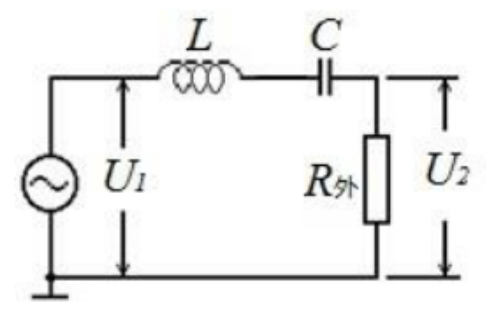
\includegraphics[width=0.5\textwidth]{../images/circuit.png}
  \caption{LCR电路}
\end{figure}

此回路中$U_2$与$U_1$的比值为
\begin{equation}
  \frac{U_2}{U_1} = \frac{R_{外}}{\sqrt{(2\pi fL-\frac1{2\pi fC})^2+R_{外}^2}}
\end{equation}
若考虑信号发生器有内阻$r$, 则这个公式应当修正为
\begin{equation}
  \frac{U_2}{U_1} = \frac{R_{外}}{\sqrt{(2\pi fL-\frac1{2\pi fC})^2+(R_{外}+r)^2}}
\end{equation}
.

品质因数的定义为电路储能与耗能的比例, 可以用电压之比表示为
\begin{equation}
  Q=\frac{U_L}{U_2}=\frac{2\pi fL}{R_{外}}=\sqrt{\frac L C}\frac{1}{R_{外}}
\end{equation}
若考虑信号发生器有内阻$r$, 则这个公式应当修正为
\begin{equation}
  Q=\sqrt{\frac L C}\frac{1}{R_{外}+r}
\end{equation}
.

\subsection{快速傅里叶变换}
傅里叶变换可以将时域信号转换为离散频域信号法, 它的定义为\cite{ft}:
\begin{equation}
  f(t)=\sum_n \mathcal F\{f\}_n e^{-i\omega_n t}
\end{equation}
其中
\begin{equation}
  \omega_n=\frac{2\pi n}{T}
\end{equation}
系数
\begin{equation}
  F\{f\}_n = \frac{1}{T}\int_0^T f(t)e^{i\omega_n t}dt
\end{equation}

方波的傅里叶变换为
\begin{align}
  F\{f\}_n=\begin{cases}
    \frac 4{\pi}\frac1{n}, & n\text{为奇数}\\
    0, & n\text{为偶数}
  \end{cases}
\end{align}
于是有级数
\begin{equation}
  f(t)=\frac 4{\pi}\sum_{n=1}^\infty \frac1{2n-1}\sin\omega_n t
\end{equation}

我们可以看到, 方波是无穷个正弦波的叠加, 这暗示我们可以利用方波打在LCR电路中, 只要做频谱的分解, 就能一次性得到$U_2/U_1$对频率的响应关系.

朴素的傅里叶变换时间复杂度为$O(N^2)$, 效率比较低, 难以应对示波器产生的百万量级的数据. 于是我们需要引入快速傅里叶变换进行优化.

快速傅里叶变换(FFT)是一种用于快速计算离散傅里叶变换(DFT)的算法, 它的计算复杂度为$O(n\log n)$, 可以快速高效地处理海量数据. 具体在实现中, 我们可以直接用Python的Numpy库的fft模块来实现快速傅里叶变换.

\section{实验过程}
由于有限周期的波在频谱上的分布是离散的, 并且频谱上频率的差值就是基频的倍数, 我们需要选取一个比较低频的方波信号来作为外源. 经过测试, 我们发现$f=530\rm{Hz}, V_{pp}=4\rm V$的方波信号表现比较良好. 

于是我们搭建了实验电路, 其中$L\approx10mH, C\approx10nF, R=500\Omega$, 接入双通道示波器, $CH1$测量$U_1$, $CH2$测量$U_2$, 得到波形图, 然后通过U盘导出时域数据(虽然示波器自带FFT功能, 但是不支持直接导出FFT后的数据)数据到电脑上以进行数据处理.

我们首先得到并绘制了CH1, CH2的时域波形图如图\ref{time_domain}.
\begin{figure}[!htbp]
  \begin{subfigure}[!t]{0.32\textwidth}
    \centering
    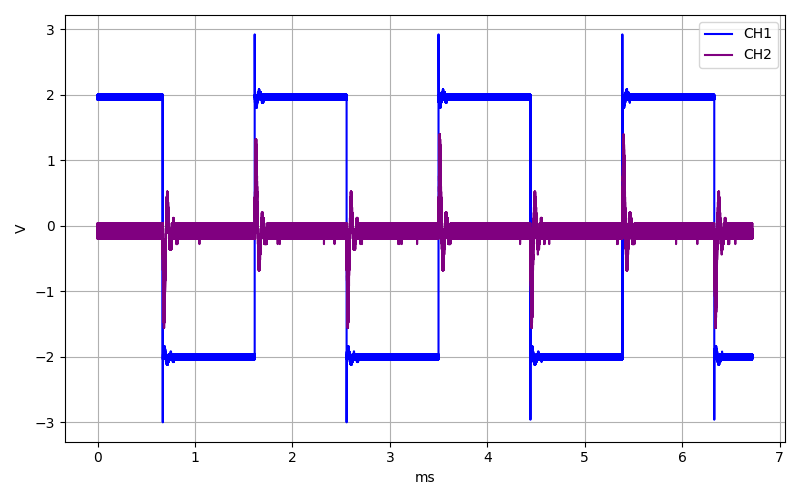
\includegraphics[width=\textwidth]{../images/fft/curve.png}
    \caption{原始波形图}\label{time_domain}
  \end{subfigure}
  \begin{subfigure}[!t]{0.32\textwidth}
    \centering
    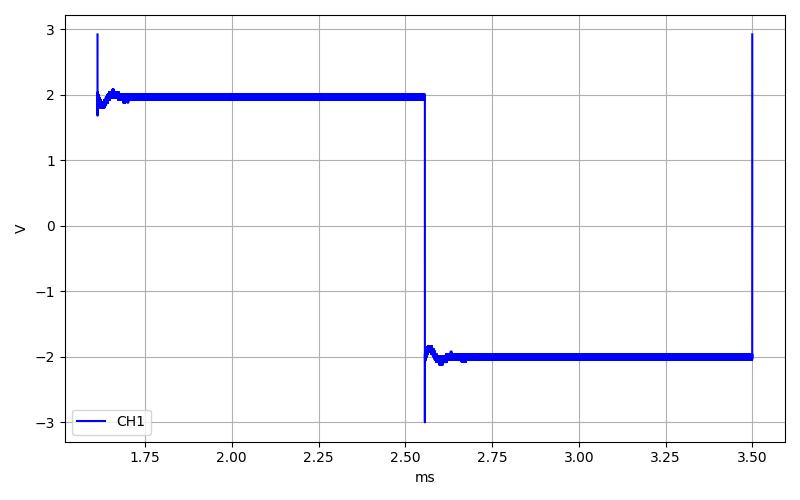
\includegraphics[width=\textwidth]{../images/fft/U1Window.png}
    \caption{$U_1\times$矩形窗口}\label{u1window}
  \end{subfigure}
  \begin{subfigure}[!t]{0.32\textwidth}
    \centering
    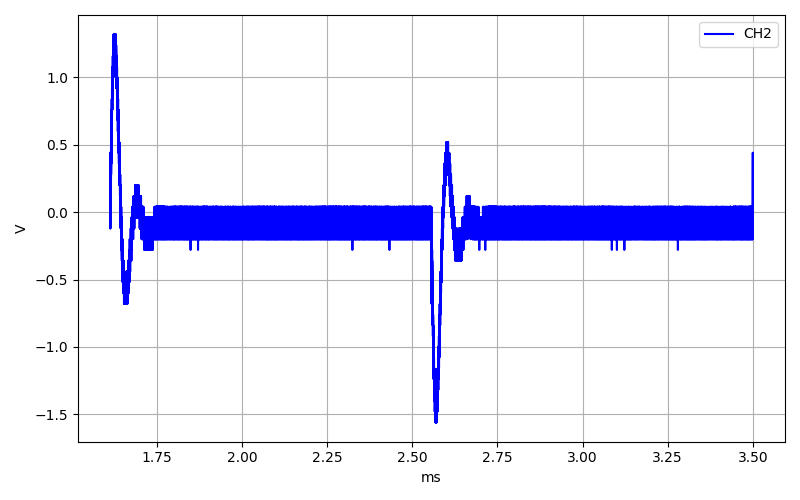
\includegraphics[width=\textwidth]{../images/fft/U2Window.png}
    \caption{$U_2\times$矩形窗口}\label{u2window}
  \end{subfigure}
  \caption{时域波形图}
\end{figure}
然后利用类似触发器的原理, 设置触发条件为上升大于$2.9V$, 获取满足这个条件的两个时间点, 在这个时间段内取矩形窗口函数对时域波形进行预处理, 如图\ref{u1window}, \ref{u2window}

然后利用FFT进行频谱分解, 得到频谱, 如图\ref{frequency_domain}. 从中我们可以清楚地看见其频率分布的离散性, 并且只有奇数倍频的傅里叶分量不为$0$. 并且从$U_2$的频谱图中, 我们已经可以通过包络线比较大概地看出频率响应曲线的形状.
\begin{figure}[!htbp]
  \centering
  \begin{subfigure}[!t]{0.4\textwidth}
    \centering
    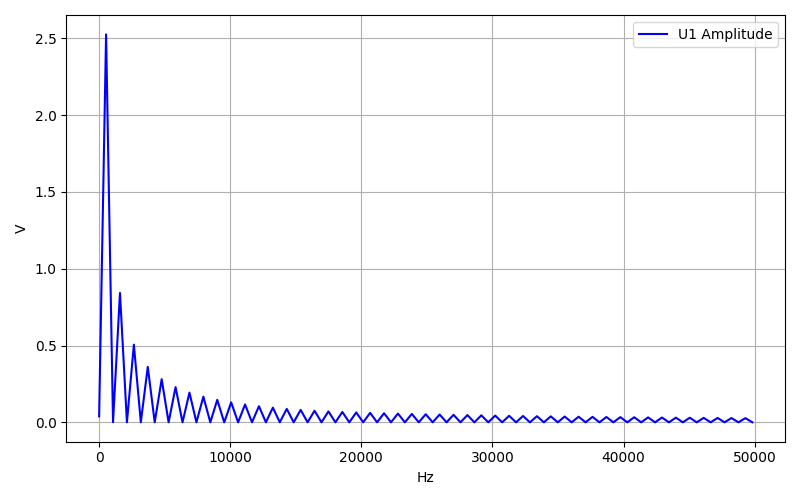
\includegraphics[width=\textwidth]{../images/fft/U1FFT.png}
    \caption{U1}\label{u1fft}
  \end{subfigure}
  \begin{subfigure}[!t]{0.4\textwidth}
    \centering
    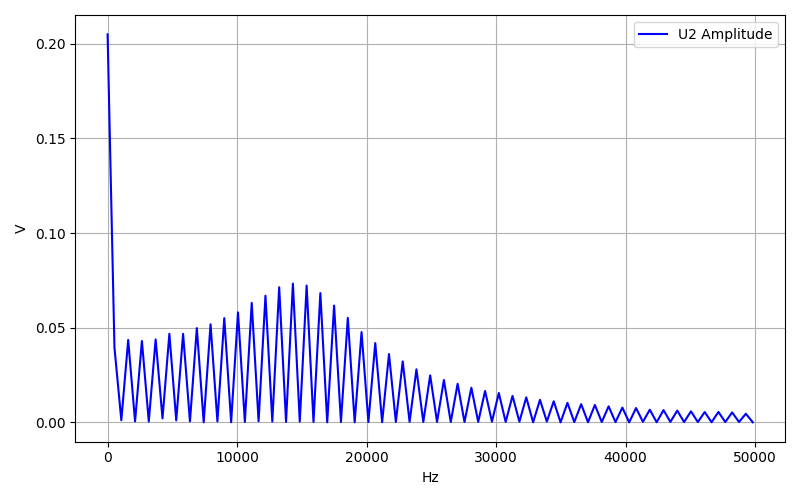
\includegraphics[width=\textwidth]{../images/fft/U2FFT.png}
    \caption{U2}\label{u2fft}
  \end{subfigure}
  \caption{频域图}\label{frequency_domain}
\end{figure}

为了方便接下来处理数据, 我们首先将偶数倍频的分量给剔除, 从而将$U_1, U_2$的频谱平滑化, 如图\ref{smooth_frequency}.
\begin{figure}[!htbp]
  \centering
  \begin{subfigure}[!t]{0.4\textwidth}
    \centering
    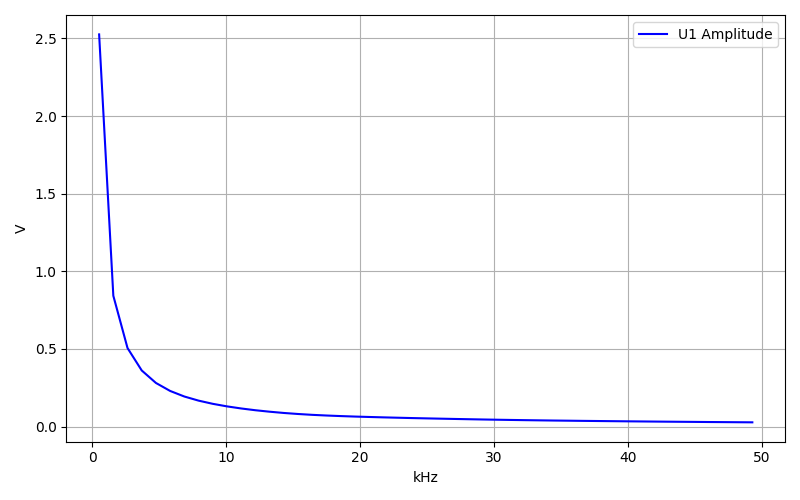
\includegraphics[width=\textwidth]{../images/fft/U1smooth.png}
    \caption{U1}\label{u1fft}
  \end{subfigure}
  \begin{subfigure}[!t]{0.4\textwidth}
    \centering
    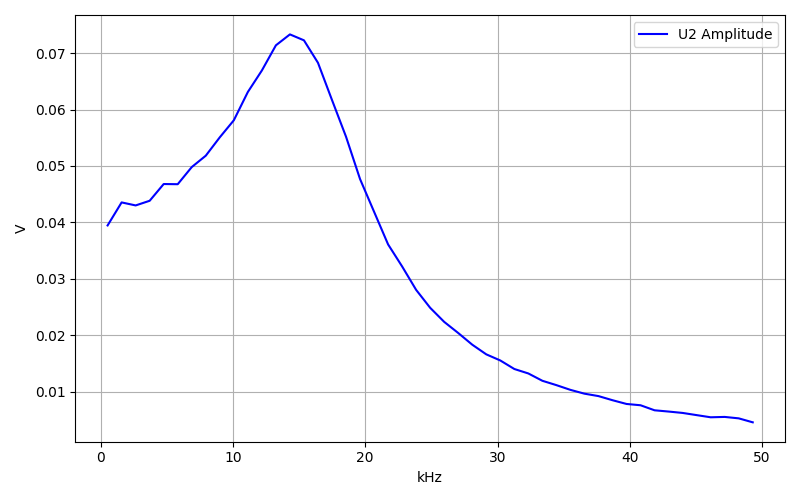
\includegraphics[width=\textwidth]{../images/fft/U2smooth.png}
    \caption{U2}\label{u2fft}
  \end{subfigure}
  \caption{平滑化频域图}\label{smooth_frequency}
\end{figure}

然后我们将$U_2$的傅里叶分量除以$U_1$的傅里叶分量, 即得到$U_2/U_1$对频率的依赖关系, 并编写Python程序对数据点进行最小二乘拟合, 得到图\ref{resonance_raw}. 其中, 模型函数选取为
\begin{equation}
  \mathcal M(f)=\frac1{\sqrt{\left(2\pi f\alpha-\frac1{2\pi f\beta}\right)^2+\gamma^2}}
\end{equation}
其中$\alpha, \beta, \gamma$为待拟合参数, 它们与$L, C, R, r$的关系为
\begin{equation}
  \alpha=\frac LR, \beta=CR, \gamma=1+\frac rR
\end{equation}
\begin{figure}[!htbp]
  \centering
  \begin{subfigure}[!t]{0.48\textwidth}
    \centering
    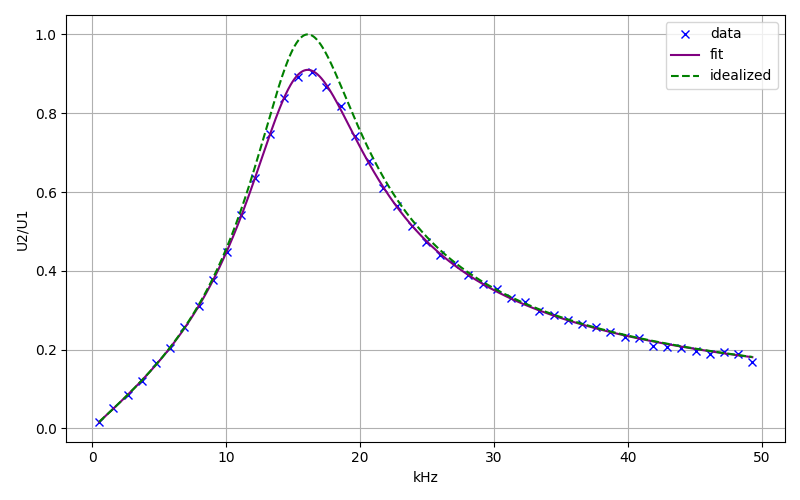
\includegraphics[width=\textwidth]{../images/fft/fitting-raw.png}
    \caption{未截取的$U2/U_1$频率响应拟合图}\label{resonance_raw}
  \end{subfigure}
  \begin{subfigure}[!t]{0.48\textwidth}
    \centering
    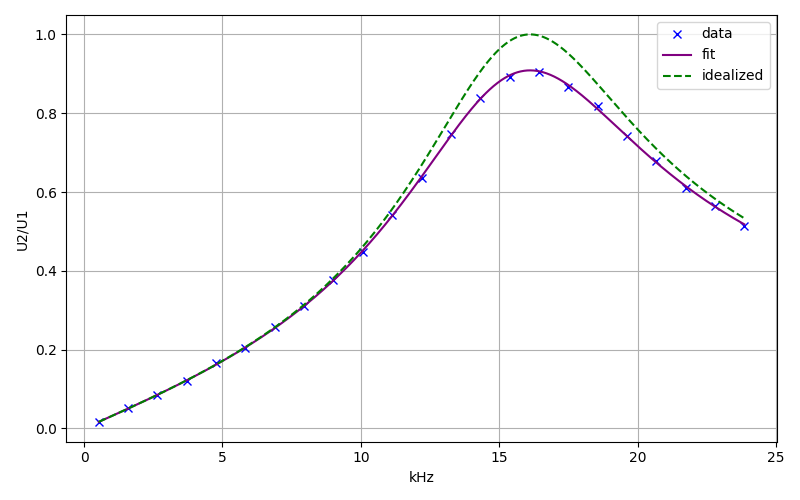
\includegraphics[width=\textwidth]{../images/fft/fitting-cutoff.png}
    \caption{截取后的$U2/U_1$频率响应拟合图}\label{resonance_cutoff}
  \end{subfigure}
  \caption{$U2/U_1$的频率响应}\label{frequency_resonance}
\end{figure}

其中, 画$\times$标记的是原始数据点, 紫色实线为拟合点, 绿色虚线为不考虑信号发生器内阻损耗时的理想情况下的$U_2/U_1-f$曲线.

但是我们发现在高频段数据浮动比较大, 拟合效果不佳, 相关系数$r$也只有$0.9998$, 因此我们尝试对频率较高区域进行了截断, 只取$0.530\rm{kHz}~23.850\rm{kHz}$, 并且重新拟合, 得到了新的拟合曲线如图\ref{resonance_cutoff}. 这次拟合的相关系数$r=0.99993$, 相较于截取前得到了优化.

于是, 根据我们最终截取后的拟合结果, 我们有测量结论电感$L=9.73(4)\rm{mH}$, 电容$C=10.02(4)\rm{nF}$, 信号发生器内阻$r=50(1)\Omega$, 谐振频率$f_0=16.11(4)\rm{kHz}$. 在$R=500\Omega$下品质因数$Q=1.79(3)$

最后, 我们将两种传统方法, 即人工反复调整正弦波频率, 利用交流电压表测量后得到的$U_2/U_1-f$曲线(如图\ref{oldfashioned}), 与方波FFT处理得到的结果进行对比, 发现两者是非常接近的, 这说明我们的方法是正确的, 可以有效地测量LCR电路的品质因数.
\begin{figure}[!htbp]
  \centering
  \begin{subfigure}[!t]{0.48\textwidth}
    \centering
    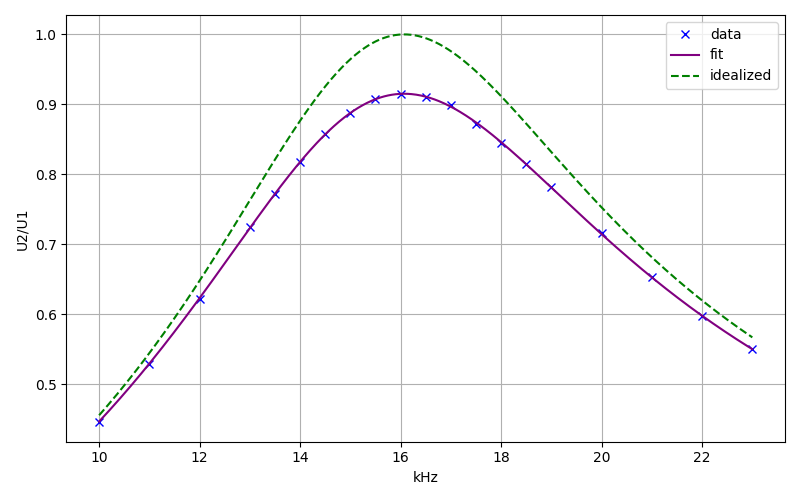
\includegraphics[width=\textwidth]{../images/meth1-fitting.png}
    \caption{固定$U_1$的$U_2/U_1-f$曲线}
  \end{subfigure}
  \begin{subfigure}[!t]{0.48\textwidth}
    \centering
    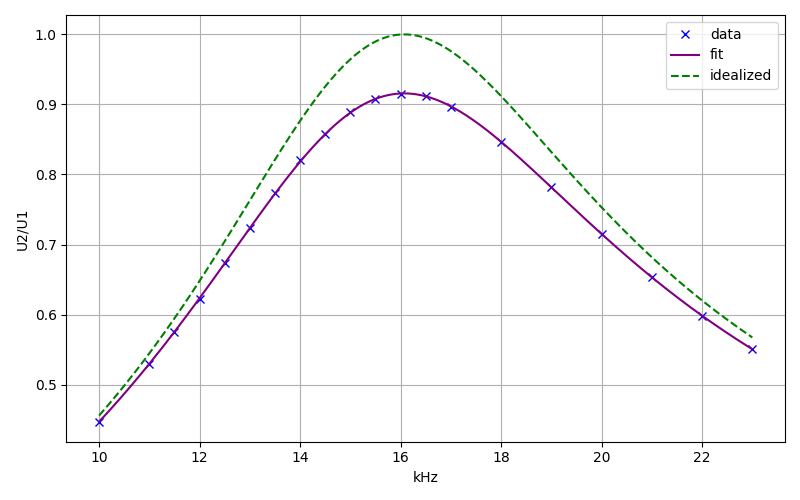
\includegraphics[width=\textwidth]{../images/meth2-fitting.png}
    \caption{固定$V_{pp}$的$U_2/U_1-f$曲线}
  \end{subfigure}
  \caption{传统方式$U2/U_1$的频率响应}\label{oldfashioned}
\end{figure}

但是, 相比之下, 由于传统方法可以选取的测量频率间隔$0.5\rm{kHz}$比方波FFT法的$1.6\rm{kHz}$小得多, 使得它在共振频率附近$U_2/U_1$的测量更为精准, 拟合的相关系数表现比方波FFT法更好(分别为$0.99997$与$0.99998$), 各个数据的不确定度也比方波FFT法要小.

\section{总结与展望}
本次实验我们创新性地提出了利用方波FFT法来对$U_2/U_1$的频率响应关系进行测量, 相比于传统方法极大地优化了操作步骤, 在牺牲精确度极小的情况下大大提高了测量效率. 

但是, 由于方波的傅里叶分量大小是随频率反比例衰减的, 这使它在高频部分(指约$25$倍于基频的部分)受杂波影响比较大, 对于测量带来了误差, 同时限制了我们不能通过进一步减小方波周期的方式来降低测量$U_2/U_1$的频率的间隔(因为此时谐振频率附近也会到大于$25$倍基频的区域, 使得信号质量降低, 反而降低测量精确度). 再加上示波器电压测量精度比交流电表低, 这使得此方法在精确度上相较于传统方法仍然存在提升空间. 

我们认为, 今后或许可以采用长周期的短脉冲信号作为外源, 这样可以减小高频部分傅里叶分量的衰减, 从而能够使得我们在减小频率间隔的情况下不损失精确度.

\printbibliography

\end{document}